% for landscape posters, use "a4paper, landscape"
\documentclass[a4paper]{article}
\usepackage{better_poster}
\usepackage[colorlinks=true, urlcolor=blue, linkcolor=red]{hyperref}


% ---- fill in from here
% poster size - this will scale the poster to the given size.
% for landscape posters add ", landscape" to the postersize command.
\postersize{a0paper}

% authors
\title{What is a hackathon?}
\author{Innovators converge to make things they aren't entirely sure how to.}

% type of poster: [exp]erimental results, [methods], [theory]
% Disclaimer: the original classification had "study" and "intervention" as separate categories. I group them under experimental results.
\newcommand\postertype{exp} % [exp],[methods],[theory]

\begin{document}

% main point of your study
\makefinding{
The \textbf{Dronecon} Hackathon hopes to gather \textbf{service members}, researchers, and partner agencies. It will be a \textbf{collider} of creative thought and real-world systems.
}


% \makemain{
% }{

% }


% the main text of your poster goes here
\makemain{
    % you can have 1 or 2 columns
    \raggedcolumns
    \begin{multicols}{2}
        \section{\underline{Who is invited?}}
        \begin{compactitem}
            \item Service members
            \item UAS enthusiasts, pilots
            \item University, Academy students
            \item Engineers, researchers
            \item Tinkerers
            \item Partner agencies
            \item Industry and small business
        \end{compactitem}
        
        \section{\underline{What, Why}}
        \begin{compactitem}
            \item Test systems in new ways
            \item Craft new equipment
            \item Hybrid warfare
            \item Information security testing
            \item Spectrum warfare
            \item Rapid prototyping
            \item New frameworks
            \item Catch up with current warfare
            \item Machine learning
            \item Automation
            \item Detection
            \item Data analytics
            \item Human performance
            \item UX/UI
        \end{compactitem}
        
    % this determines where your columns will be separated
    \columnbreak

        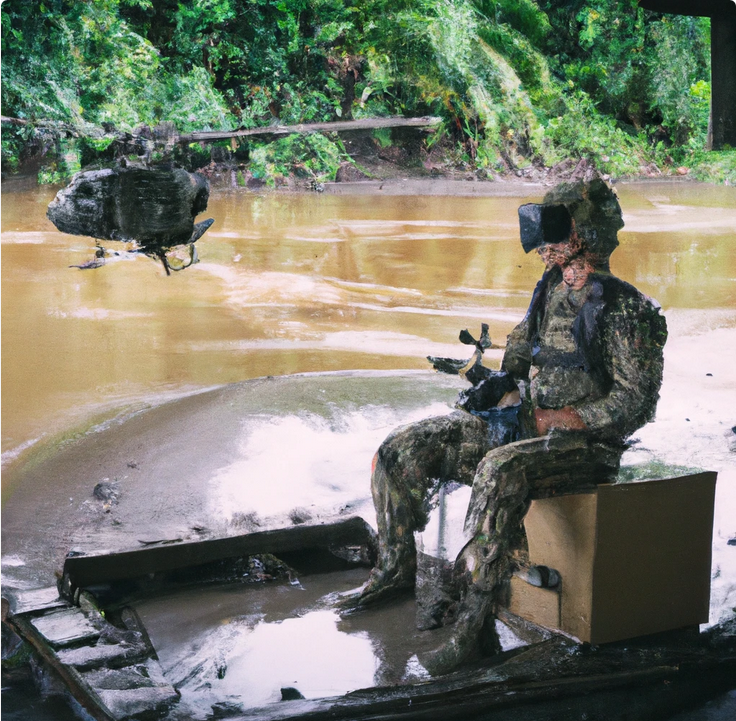
\includegraphics[width=\linewidth]{images/green-man.jpg}
        
		\section{\underline{How do I get involved?}}

			
		\begin{compactitem}
			\item Complete the \href{https://forms.office.com/r/6H6wFBtK5a}{interest form}
			\item Apply to a \href{https://bravo.il2.afwerx.dso.mil/}{BRAVO Hackathon}
			\item Become a \href{https://www.tesseract.af.mil/Network/}{Tesseract LNO} \newline
                \item Visit \href{https://dronecon.net}{dronecon.net}
                \item visit \href{https://dronewa.rs/details}{dronewa.rs}
                \item Follow us on \href{https://www.linkedin.com/company/dronecon-hackathon/}{LinkedIn}
                \item Check out our \href{https://github.com/orgs/Dronewa-rs/repositories}{Github} repos

		\end{compactitem}
    
    \end{multicols}
}
% If you have extra figures or data to show
\makeextracolumn{
    
    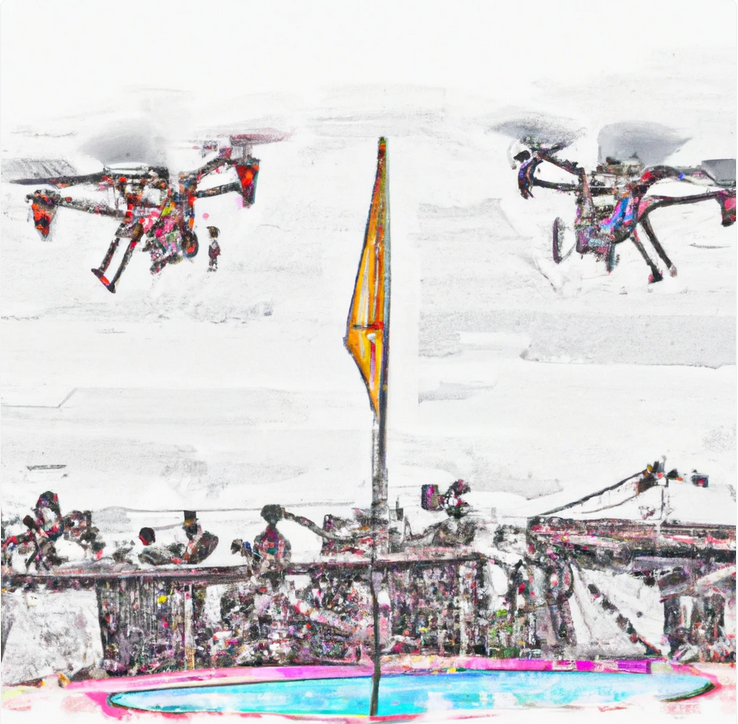
\includegraphics[width=0.5\linewidth]{images/flags2.jpg}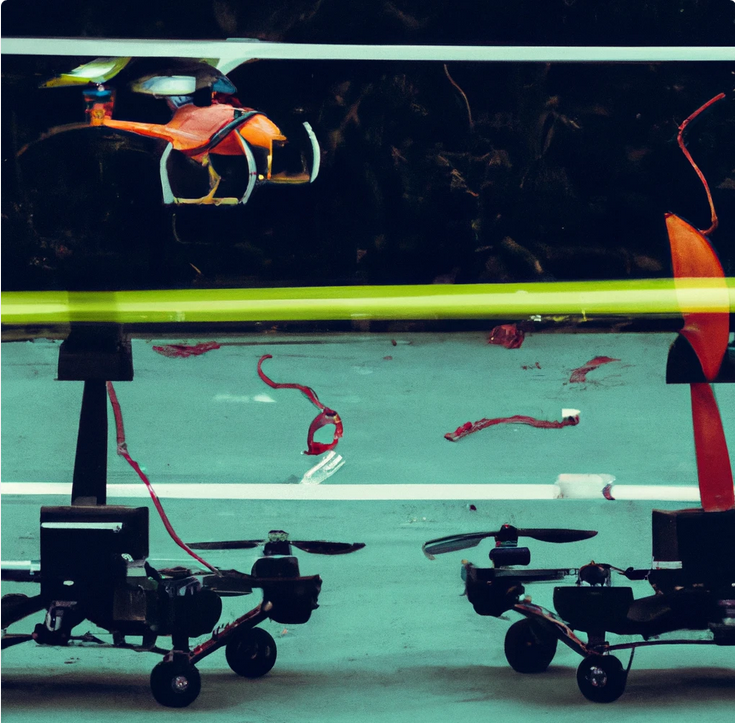
\includegraphics[width=0.5\linewidth]{images/tennis-field.jpg} \newline
    
    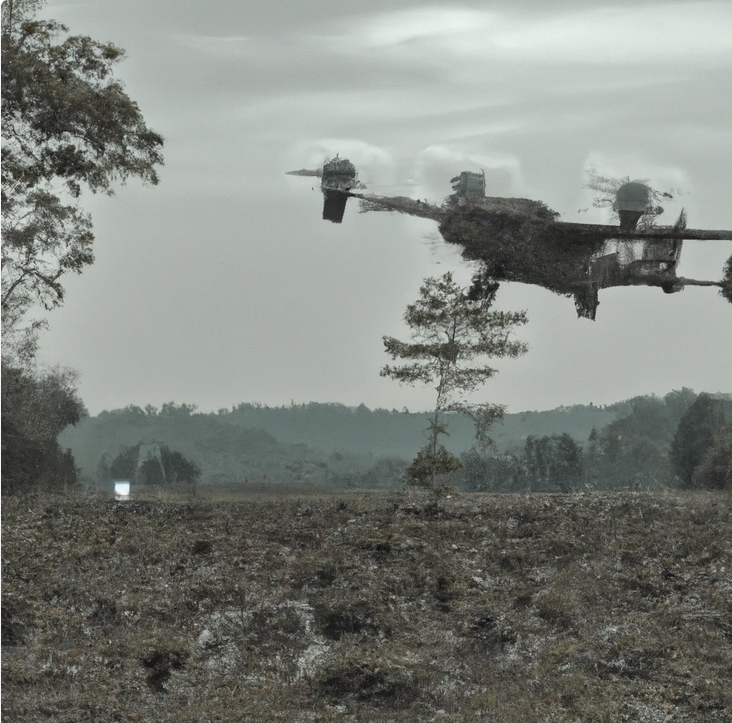
\includegraphics[width=0.5\linewidth]{images/nam.jpg}\includegraphics[width=0.5\linewidth]{thumb-nam.png} \newline
    
    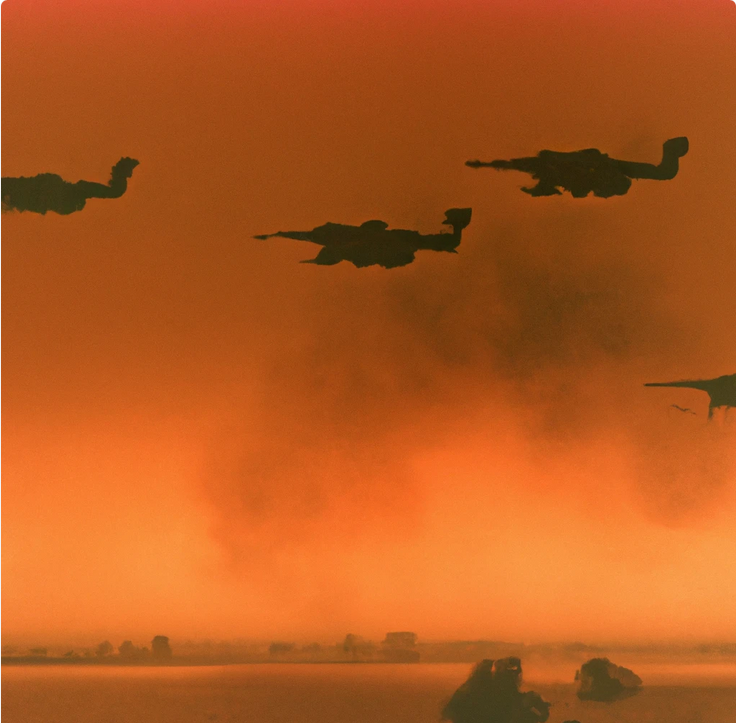
\includegraphics[width=0.5\linewidth]{images/nyoom.jpg}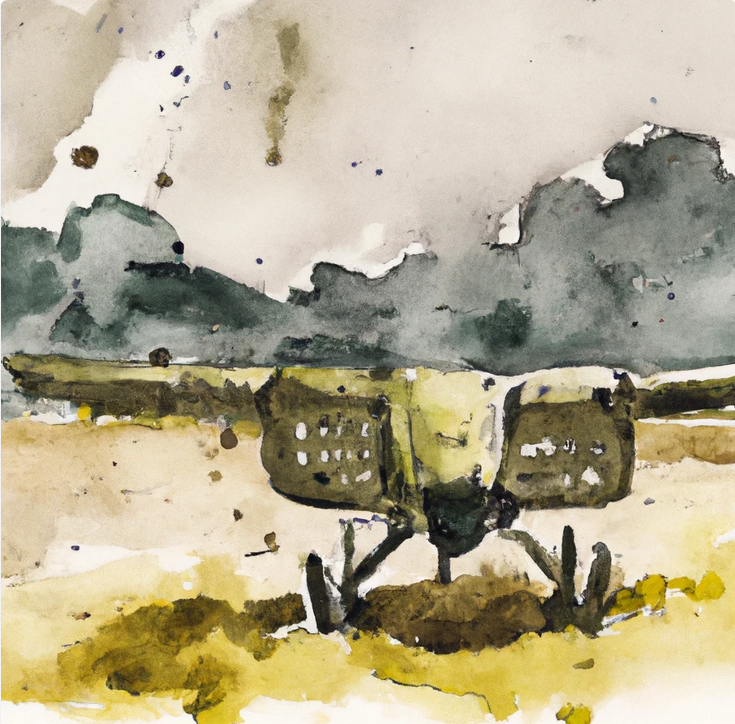
\includegraphics[width=0.5\linewidth]{images/flack.jpg} \newline
    
    \includegraphics[width=0.5\linewidth]{thumb-mud-2.png}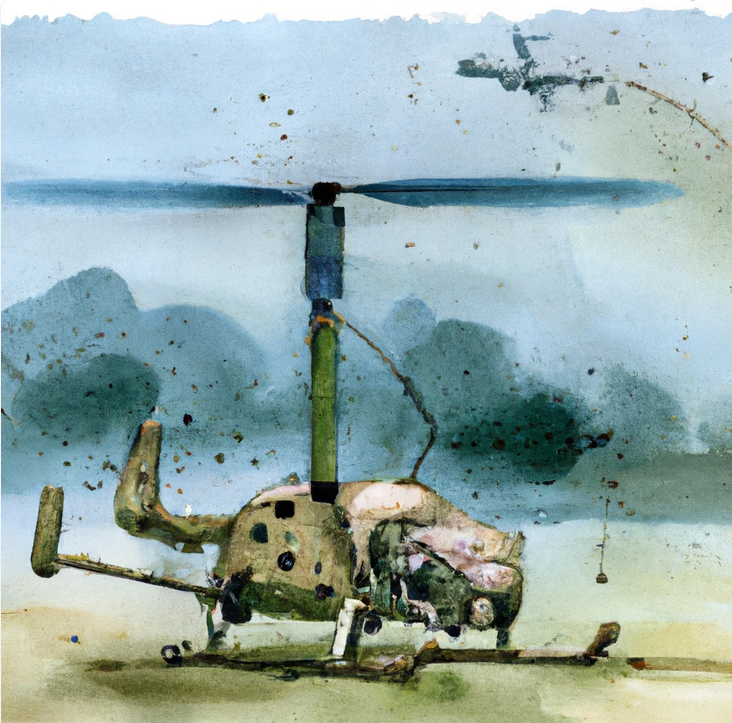
\includegraphics[width=0.5\linewidth]{images/chopper.jpg} \newline 
    
    \huge{\textbf{See you there!}}
    
}


% footer
% generate qr code from https://www.qr-code-generator.com/ and replace qr_code.png
% default: barcode on the left
\makefooter{images/dronewars.png}{images/dronecon.png}{dronecon.net}{dronewa.rs}
% replace with this like for barcode on the right
%\makealtfooter{images/uni_logo.png}{images/qr-code.png}
 
\end{document}